\documentclass[12pt, a4paper]{article}

% Ru lang stuff
\usepackage [utf8x] {inputenc}
\usepackage [T2A] {fontenc}

% running titles 
\usepackage{fancybox}
\usepackage{fancyhdr}

% for last page number
\usepackage{lastpage}

%for colored tablets cells
\usepackage{colortbl}

% for Ru text in formulas
\usepackage[warn]{mathtext}

% for captions 
\usepackage[labelsep=period]{caption}
\usepackage{capt-of}

% for colored hyperrefs
\usepackage{xcolor}
\usepackage{hyperref}

% for pictures 
\usepackage{graphicx}

% for coll math
\usepackage{amsmath}

% path to all pictures
\graphicspath{{picks/}}

% for enumerates
\usepackage[shortlabels]{enumitem}

% for diff running titles on pages with diff parity
\usepackage{ifthen}
\usepackage{pdfpages}
\usepackage[strict]{changepage}

% for graphics
\usepackage{pgfplots}
\pgfplotsset{compat=1.9}

%for drawings
\usepackage{tikz}
\usetikzlibrary{calc}
\usetikzlibrary{decorations.pathmorphing}

% for good text in tablets
\usepackage{array}

% upgrading tables
\newcolumntype{P}[1]{>{\centering\arraybackslash}p{#1}}
\newcolumntype{M}[1]{>{\centering\arraybackslash}m{#1}}


% dock fields 20 15 15 35
\usepackage[left=12mm, top=12mm, right=15mm, bottom=28mm, nohead, footskip=10mm]{geometry}

% for cool tables
\usepackage{multirow}

% for different section/subsection/subsubsection styles in contents and doc
\usepackage[english, russian]{babel}

\usepackage{amsmath}

% for cool tables
\usepackage{tabularx}

\newcommand{\sect}[2] {
    \addtocounter{section}{1}
    \section*{\Huge\thesection.\,#1}
    \addcontentsline{toc}{subsection}{ \texorpdfstring{\thesection.\qquad\qquad #2}{Lg}}
}

\newcommand{\subsec}[2] {
    \addtocounter{subsection}{1}
    \subsection*{\thesubsection.\,#1}
    \addcontentsline{toc}{subsection}{ \texorpdfstring{\quad \thesubsection.\qquad\ #2}{Lg}}
}

\newcommand{\subsubsec}[2] {
    \addtocounter{subsubsection}{1}
    \subsubsection*{\thesubsubsection.\,#1}
    \addcontentsline{toc}{subsection}{ \texorpdfstring{\quad\quad\ \thesubsubsection. #2}{Lg}}
}
%-------------------------------------------------------------------------%

% for easy mini pages with shifts
\newcommand{\shiftedText}[3]{
\hspace*{#1}\begin{minipage}[t]{#2}
#3
\end{minipage}
}

\newcolumntype{P}[1]{>{\centering\arraybackslash}p{#1}}

% page style setup (for running titles)
\fancypagestyle{plain}{ %
\fancyhf{} % remove everything

 % lines parameters
\renewcommand{\headrulewidth}{0pt}
\renewcommand{\footrulewidth}{0pt}

% running titles contents
\fancyfoot[L]{\ifthenelse{\isodd{\thepage}}{Работа 1.3.2}{\thepage}}
\fancyfoot[R]{\ifthenelse{\isodd{\thepage}}{\thepage}{Работа 1.3.2}}
}

% choosing page style with our running titles
\pagestyle{plain}

\tolerance = 10000

\title{Лабораторная работа №1.3.2}
\author{Mikhail Pavlov \thanks{MIPT}}
\date{December, 2021}
\begin{document}


\shiftedText{0.5cm}{14cm}
{
    \begin{center}
    \vspace*{1.0cm}    
        
        {\bf\Huge Работа 1.3.2 }
        
    \vspace*{0.2cm}    
        
        {\bf\LARGE Определение модуля Юнга по измерениям растяжения проволоки. }
        
    \vspace*{0.8cm}
        {\LARGE Работу выполнил Павлов Михаил Б01-109 }
        
    \vspace*{1.6cm}
    
    \end{center}
}

\fancypagestyle{plain}{ %
\fancyhf{} % remove everything

 % lines parameters
\renewcommand{\headrulewidth}{0pt}
\renewcommand{\footrulewidth}{0pt}
% running titles contents
\fancyfoot[L]{\ifthenelse{\isodd{\thepage}}{Работа 1.3.2}{\thepage}}
\fancyfoot[R]{\ifthenelse{\isodd{\thepage}}{\thepage}{Работа 1.3.2}}
}

% choosing page style with our running titles
\pagestyle{plain}

\tolerance = 10000

\vspace*{0.6cm}

{\Large 1. Аннотация \\}

\vspace{1cm}
{\Large 2. Теоретические сведения \\}

При закручивании цилиндрических стержней круглого сечения распределение деформаций и напряжений одинаково по длине стержня только вдали от мест. где прикладываются моменты сил. Для этих областей можно считать, что каждое поперечное сечение поворачивается как жёсткое, то есть частички материала не сходят с тех радиальных линий, на которых они находились вначале, и все эти радиальные линии поворачиваются на один и тот же угол.

Напряжённое состояние, которое возникает в стержне, называется кручением.

Рассмотрим часть закручиваемого круглого цилиндра, имеющую длину $l$ (см. рис 1). Любая прямая линия, проведённая до закручивания цилиндра по частицам материала и параллельная оси симметрии, при закручивании превращается в спираль. Сечения, находящиеся на расстонии $l$, повёрнута на угол $\varphi$.

Рассмотрим в цилиндре колечко произвольного радиуса $r$ с бесконечно малой толщиной $dr$ и бесконечно малой высотой $dl$. При закручивании верхнее сечение колечка поворачивается относительно нижнего на угол $d\varphi$, а образующая цилиндрической поверхности колечка $dl$ наклоняется на угол $\alpha$, представляя элемент тех спиральных линий, о которых говорилось выше. При небольших углах $\alpha$ можно написать
\[\alpha dl = r d\varphi\]

По закону Гука касательное напряжение $\tau$ связано с углом сдвига $\alpha$ линейной зависимостью, в которую входит модуль сдвига $G$:
\[\tau = G \alpha\]

Комбинируя две последние записанные формулы, имеем:
\[\tau = G \alpha = G r \frac{d\varphi}{d l}\]

Касательное напряжение создаёт момент сил относительно оси цилиндра:
\[dM = \tau dS  r = 2 \pi r dr \tau r = 2 \pi G \frac{d\varphi}{d l} r^3 dr\]

Суммарный момент сил, действующий на всём поперечном сечении цилиндра, равен

\[M = \int_M dM = \int_0^{R}2 \pi G \frac{d\varphi}{d l} r^3 dr = \pi G \frac{d\varphi}{d l} \frac{R^4}{2}\]

Так как стержень находится в равновесии, то момент, записанный выше, постоянен, значит постоянно и выражение
\[\frac{d\varphi}{d l} = const \Rightarrow \varphi = const \cdot l \text{ (с учётом граничных условий)}\]

\[M = \frac{\pi G R^4}{2l} \varphi = f \varphi\]

Здесь была введена вспомогательная величина $f$ -- модуль кручения. 

Следует отметить, что полученная формула справедлива только малых значений касательного напряжения.\\


\vspace{1cm}
{\Large 3. Инструментальные погрешности \\}
\noindent
\textbf{Линейка: } $\sigma_{rul} = \pm 0.5$ мм (половина цены деления)\\
\textbf{Микрометр: } $\sigma_{mic} = \pm 0.01$ мм (маркировка производителя) \\
\textbf{Весы: } $\sigma_{m} = \pm 0.1$ г (маркировка производителя) \\
\textbf{Секундомер: } $\sigma_{sw} = \pm 0.01$ c (маркировка производителя) \\


{\Large 4. Экспериментальная установка \\}

\noindent\begin{minipage}[c]{0.53\textwidth}
    \hspace{1cm}
    Экспериментальнеая установка (см рис.), используемая в этой части, состоит из длинной вертикально висящей проволоки П, к нижнему концу которой прикреплён горизонтальный металлический стержень С с двумя симметрично расположенными грузами Г. 
    Их положение не стержне можно фиксировать. Верхний конец проволоки зажат в цангу и при помощи специального приспособления может вместе с цангой поворачиваться вокруг вертикальной оси. 
    Таким способом в системе можно возбуждать крутильные колебания. 
    

\end{minipage}
\begin{minipage}[c]{0.42\textwidth}
    \begin{center}
        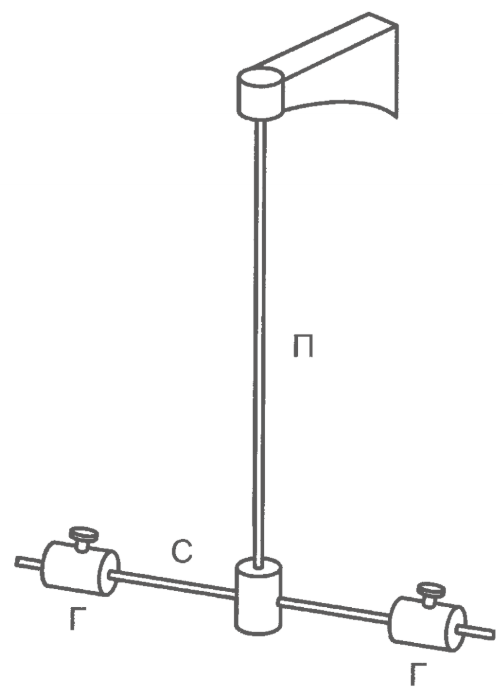
\includegraphics[scale=0.42]{Pics/picture1.png} \\
        \textit{\textcolor[HTML]{000000}{Рис. 1. Экспериментальная установка}}
    \end{center}
\end{minipage}  

\vspace*{0.3cm}
{\Large 5. Результаты измерений и обработка данных \\} 

Вращение стержня С с закреплёнными на нём грузами Г вокруг вертикальной оси происходит под действием упругого момента, возникающего в проволоке. Оно описывается уравнением
\[I \frac{d^2 \varphi}{d t^2} = -M = -f \varphi\]

Здесь $I$ -- момент инерции стержня с грузами относительно оси вращения, $\varphi$ -- угол поворота стержня от положения равновесия, а $M$ -- момент сил, действующий на стержень. 

Полученное дифференциальное уравнение имеет решение
\[\varphi = \varphi_0 sin(\omega t + \theta)\]

Здесь начальная фаза $\theta$ и амплитуда колебаний $\varphi_0$ задаются начальными условиями, а $\omega = \sqrt{\frac{f}{I}}$.

Период колебаний равен 
\[T = 2 \pi \sqrt{\frac{I}{f}} \]

Теперь важно понять, что уравнение движения было составлено без учёта диссипативных сил, соответственно было получено решение для незатухающий колебаний. Но в этом ещё надо убедиться: для оценки можно положить, что рассматриваемые колебания действительно незатухающие, если логарифмический декремент затухания меньше, чем $0,1$:
\[\lambda = ln\frac{\varphi (t)}{\varphi (t + T)} = \frac{1}{N} < \frac{1}{10} \Rightarrow N > 10\]

Здесь $N$ -- количество колебаний, за которое амплитуда уменьшается в $e$ раз. Вывод записанной формулы следует из уравнения затухающих колебаний.

Для начала установим диапазон амплитуд, в котором применимы результаты, полученные для незатухающий колебаний, в частности независимость периода колебаний от амплитуды. Для этого укрепим грузы на некотором расстоянии от проволоки и возбудим в системе крутильные колебания. Измерив порядка $10$ периодов колебания для некоторой выбранной амплитуды, находим этот период колебания $T_1$. Теперь находим таким же способом период колебаний $T_2$, где амплитуда колебаний в два раза меньше. Если периоды совпадают, то будем брать амплитуды не больше выбранной, если не совпадают, то берём более мелкую амплитуду и повторяем действия.  

Теперь убедимся в том, что логарифмический декремент затухания больше меньше $1/10$. Зафиксируем начальную амплитуду и посмотрим, как она поменяется спустя $10$ колебаний. Получаем, что амплитуда изменил меньше, чем в 2 раза, значит она тем более изменилась меньше, чем в $e$ раз.

Меняя расстояние от начала оси до грузов $l$, будем измерять период колебаний системы $T$. Каждое имзерение проводим $2$ раза. Запишем все данные в таблицу:

\begin{center}
\begin{tabular}{|c|c|c|c|c|c|c|}
\hline 
$l$, см & 5.4 & 7.4 & 8.8 & 10.3 & 12.0 & 13.5 \\ 
\hline 
$T$, с & 47.38 & 43.05 & 48.91 & 54.31 & 61.12 & 66.78 \\ 
\hline 
$T$, с & 47.56 & 43.04 & 48.69 & 54.59 & 61.03 & 66.40 \\ 
\hline 
\end{tabular}
\end{center} 

В данном случае можно провести следующую линеаризацию:
\[T^2 = \frac{4\pi^2 I}{f}\]

Момент инерции из-за больших размеров грузов сильно меняется, поэтому использовать аппроксимацию материальной точки нельзя. Нужно посчитать момент инерции для каждой длины. 

Для начала выведем формулу для момента инерции. Начнём с того, что выведем момент инерции для диска радиуса $R$, находящегося на расстоянии $l$ от рассматриваемой оси:

\[dm = \sigma dS = \sigma 2\pi r dr = \frac{m}{\pi R^2} 2\pi r dr = \frac{2m}{R^2} r dr\]
\[I = \int_{I} (r^2 + l^2) dm = \frac{2m}{R^2}\Big(\int_{0}^{R} r^3 dr + l^2\int_{0}^{R} r dr \Big) = \]
\[= \frac{m}{R^2}\Big(\frac{R^4}{2} + l^2 R^2 \Big) = m\Big(\frac{R^2}{2} + l^2 \Big)\]

Теперь представим, что мы рассматриваем бесконечно тонкий диск толщиной $dl$, значит для него выполняется
\[dI = dm\Big(\frac{R^2}{2} + l^2 \Big) = \frac{m}{L} dl\Big(\frac{R^2}{2} + l^2 \Big) \]
\[I = \frac{m}{L} \int_{l}^{l+L} \Big(\frac{R^2}{2} + l^2 \Big) dl = \frac{m}{L} \Big(\frac{L R^2}{2} + \int_{l}^{l+L} l^2 dl \Big) = \frac{m}{L} \Big(\frac{L R^2}{2} + \frac{(l+L)^3 - l^3}{3} \Big) \]
\[I = \frac{m}{L}\Big(\frac{R^2 L}{2} + \frac{1}{3}\big((l + L)^3 - l^3\big)\big)\]

Для нашей ситуации надо брать в расчёт два груза  ещё нужно учесть, что у системы есть собственный момент инерции, тогда
\[I = \frac{2m}{L}\Big(\frac{R^2 L}{2} + \frac{1}{3}\big((l + L)^3 - l^3\big)\big) +  I_0 = I_1 + I_0\]

Здесь у нас $l$ -- расстояние от оси до цилиндра, $L = 4$ см -- длина самого цилиндрического груза, $R = 2$ см -- радиус цилиндрического груза, а $m = 375$ г -- масса цилиндрического груза, $I_0$ -- момент инерции системы без грузов.

Найдём собственный момент инерции системы. Для этого посчитаем период колебаний системы без грузов:

\begin{center}
\begin{tabular}{|c|c|c|}
\hline 
$T$, с & 1,120 & 1,115 \\ 
\hline 
\end{tabular}
\end{center} 

Найдём среднюю величину $\langle T \rangle = 1,117$. Также полезным будет значение $\langle T \rangle^2 = 1,25 \text{ с}^2$. Для собственного момента инерции имеем:
\[I_0 = \frac{\langle T \rangle^2}{4\pi^2}f\]

Значит формула для периода колебаний выглядит так:
\[T^2 = \frac{4\pi^2 (I_1 + I_0)}{f} = T^2 = \frac{4\pi^2 I_1}{f} + \langle T \rangle^2 \Rightarrow T^2 - \langle T \rangle^2 = \frac{4\pi^2 I_1}{f}\]

Строим таблицу для моментов инерции в зависимости от $l$, попутно считая средние значения для периода колебаний:\\

\begin{center}
\begin{tabular}{|c|c|c|c|c|c|c|}
\hline 
$l$, см & 5.4 & 7.4 & 8.8 & 10.3 & 12.0 & 13.5 \\ 
\hline 
$I_1 \cdot 10^{-3}$, $\text{кг} \cdot \text{м}^2$  & 3,179 & 4,192 & 5,355 & 6,667 & 8,130 & 9,742 \\ 
\hline 
$T$, с & 2.37 & 2.87 & 3.25 & 3.63 & 4.07 & 4.44 \\ 
\hline 
$\Delta T$, c & 0,014 & 0,010 & 0,017 & 0,019 & 0,012 & 0,023 \\ 
\hline
$T^2$, $\text{с}^2$ & 5.62 & 8.24 & 10.56 & 13.18 & 16.56 & 19.71 \\ 
\hline 
$\Delta (T^2)$, $\text{с}^2$ & 0,08 & 0,06 & 0,07 & 0,09 & 0,08 & 0,12 \\ 
\hline 
\end{tabular}
\end{center}   

Сразу считаем значения для линеаризации $T^2$, $l^2$, $(\Delta T)^2 = 2 T \Delta T$. Строим график зависимости $T(l)$ и с помощью метода хи-квадрат считаем, чему равен коэффициент линеаризации и его погрешность:

\begin{center}
    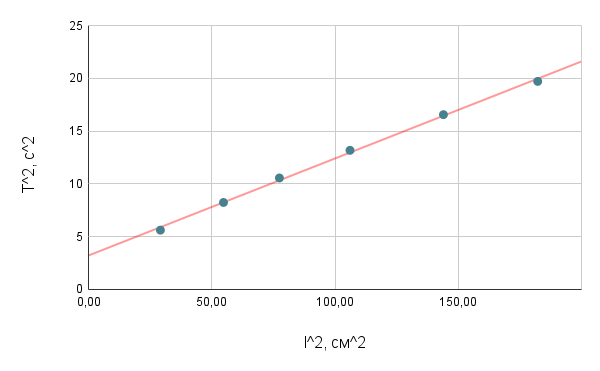
\includegraphics[scale=0.82]{Pics/picture2.png} \\
    \textit{\textcolor[HTML]{000000}{Рис. 2. График зависимости $T^2$ от $l^2$}}
\end{center}

\[\frac{4\pi^2}{f} = \frac{\langle (T^2 - \langle T \rangle^2) I \rangle^{'}}{\langle I^2 \rangle^{'}} = \frac{\sum_{i = 1}^{7} \frac{(T^2 - \langle T \rangle^2)_i}{(\Delta (T^2 - \langle T \rangle^2))^2} I_i}{\sum_{i = 1}^{7} \frac{I^2_i}{(\Delta (T^2 - \langle T \rangle^2))^2}} = \]
\[= 1,072 \cdot 10^3 \text{ Н}^{-1} \cdot \text{м}^{-1}\]
\[f = 5,392 \cdot 10^{-2}\text{ Н} \cdot \text{м}\]

\[\Delta \Big(\frac{4\pi^2}{f}\Big) =  \frac{\Delta f}{f} \frac{4\pi^2}{f} = \sqrt{\frac{1}{6}\Big( \frac{\langle (T^2 - \langle T \rangle^2)^2 \rangle}{\langle I^2 \rangle} - \Big(\frac{4\pi^2}{f}\Big)^2\Big)} = \]
\[= 18,28 \text{ Н}^{-1} \cdot \text{м}^{-1}\]

\[\Delta f = 6,27 \cdot 10^{-4}\text{ Н} \cdot \text{м}\]

Теперь измерим длину и диаметр стержня:
\begin{center}
\begin{tabular}{|c|c|c|c|c|c|c|c|c|}
\hline 
$L$, см & 144,1 & 144,1 & 144 & 144,2 & 144 & 144 & 144,2 & 144 \\ 
\hline 
$D$, мм & 1,91 & 1,92 & 1,91 & 1,92 & 1,91 & 1,91 & 1,91 & 1,92  \\ 
\hline 
\end{tabular}
\end{center} 

Значит, для длины и диаметра имеем: $L_0 = 1,74$ м, $\Delta L_0 = 0,0001$ м, $D = 1,98$ мм, $\Delta D = 0.01 \text{ мм}$ 

Теперь посчитаем модуль сдвига и его погрешность:
\[G = \frac{2fL_0}{\pi R^4} = 3.824 \cdot 10^{10}\text{ Н} \cdot \text{м}^{-2}\] 
\[\Delta G = G \sqrt{\Big( \frac{\Delta f}{f}\Big) ^2 + \Big(\frac{\Delta L_0}{L_0} \Big)^2 + \Big(4\frac{\Delta R}{R} \Big)^2}= 8,91 \cdot 10^8 \text{ Н} \cdot \text{м}^{-2}\]

    \underline{Окончательный результат:} G = $3.824 \pm 0.089 \cdot 10^{10}$ Па \\ 


    \vspace*{0.3cm}
    {\Large 6. Вывод \\} 

В результате эксперимента определили модули кручения и сдвига для проволоки по измерениям крутильных колебаний подвешенного на ней маятника (динамическим методом). 

Сравним полученные значения модуля сдвига с табличными: значение совпадает с модулем сдвига меди ($3,5-4,9 \cdot 10^{10}\text{ Н} \cdot \text{м}^{-2}$).


\end{document}